\clearpage

\paragraph{Soggetto 1}~

Per verificare le prestazioni e il funzionamento dei moduli progettati, sono state effettuate alcune misurazioni su un soggetto maschio, di età 55 anni, di carnagione chiara. Il soggetto si trovava in condizioni di riposo.

\paragraph{MAX86916}~

Di seguito sono riportati i risultati ottenuti utilizzando il sensore MAX86916.

\subparagraph{Polpastrello indice sinistro}

Il polpastrello rappresenta il sito di misura più utilizzato poiché permette di ottenere ottimi segnali PPG ed è facilmente indossabile. Come si può notare in figura \ref{fig:soggetto1_polpastrello}, tutte le misurazioni presentano una buona e distinguibile componente AC. Infatti, è possibile distinguere sia il picco sistolico sia il picco diastolico anche con la luce verde e blu. Le acquisizioni con la luce verde e blu presentano un andamento più \textit{smooth}. Questa caratteristica è determinata dalla minore penetrazione della luce verde-blu, che rende le misurazioni meno soggette ad interferenze dovute a movimenti, anche minimi, del soggetto. La figura rappresenta il segnale PPG nell'arco di 10 secondi. Contando i picchi presenti, e moltiplicandoli per un fattore 6, è possibile effettuare una stima della frequenza cardiaca del soggetto. In questa misurazione, si possono individuare 12 picchi, stimando una frequenza cardiaca di 72 battiti al minuto.\todo{componente dc}

\begin{figure}[h]
	\centering
	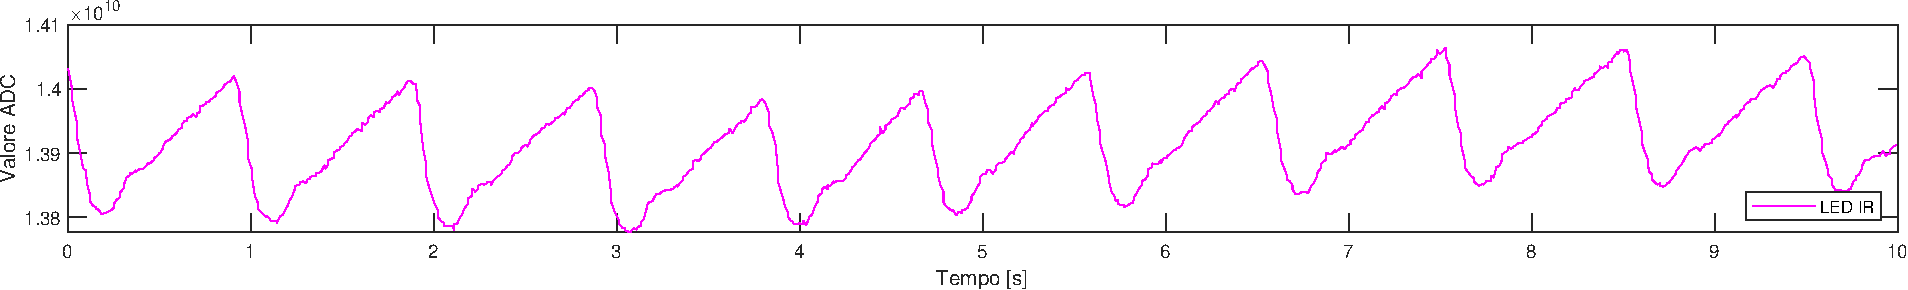
\includegraphics[width=1\linewidth]{ImageFiles/Misure Preliminari/Soggetto 1/polpastrello_ired}
	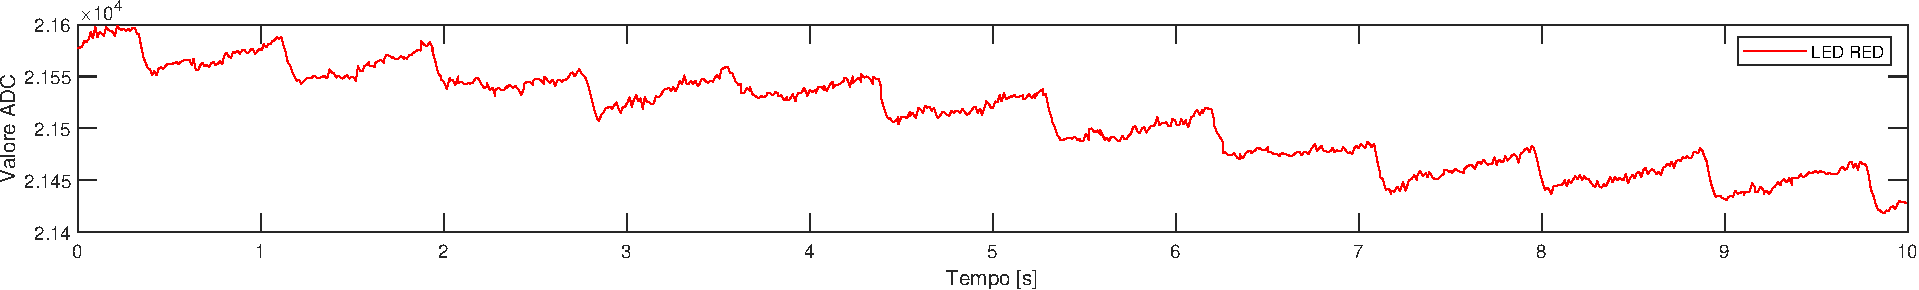
\includegraphics[width=1\linewidth]{ImageFiles/Misure Preliminari/Soggetto 1/polpastrello_red}
	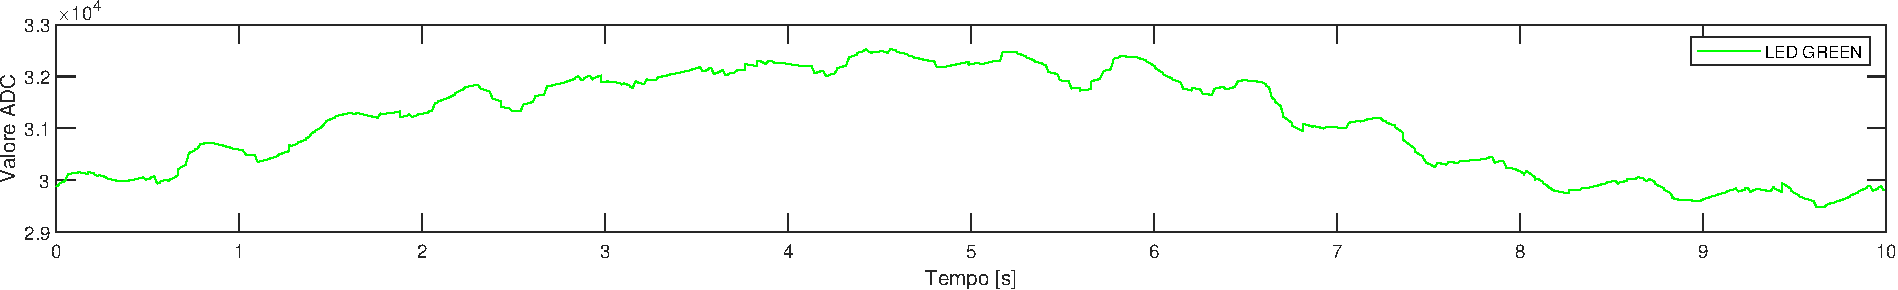
\includegraphics[width=1\linewidth]{ImageFiles/Misure Preliminari/Soggetto 1/polpastrello_green}
	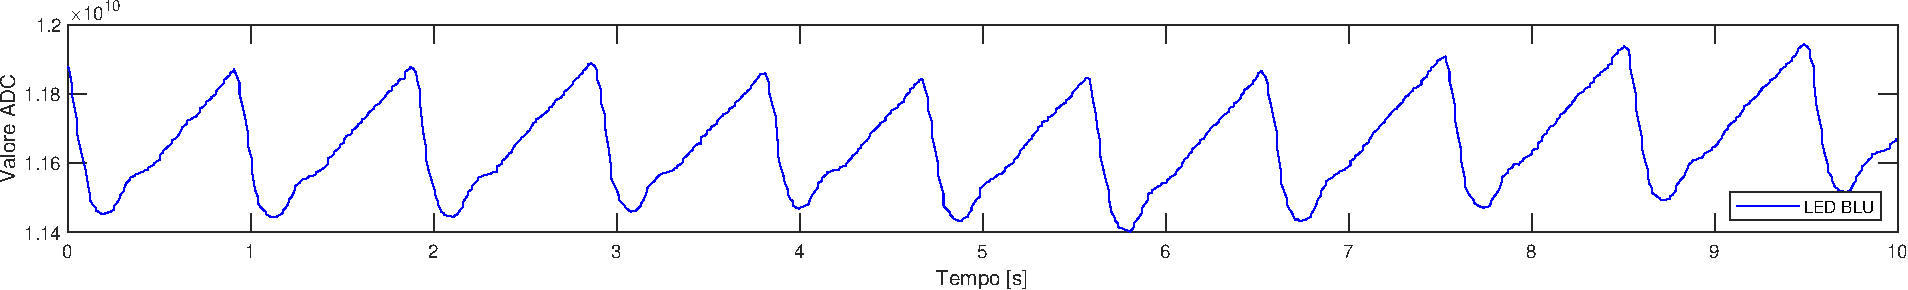
\includegraphics[width=1\linewidth]{ImageFiles/Misure Preliminari/Soggetto 1/polpastrello_blu}
	\caption{Segnali PPG acquisiti sul polpastrello del dito indice sinistro.}
	\label{fig:soggetto1_polpastrello}
\end{figure}

\clearpage

\subparagraph{Lobo orecchio destro}

In figura \ref{fig:soggetto1_lobo} sono riportate le misurazioni effettuate sul lobo dell'orecchio destro. I segnali risultano buoni anche in questo sito di misura con tutte e quattro i LED. Utilizzando il prototipo realizzato, il sito non è risultato comodo per effettuare le misurazioni. Tuttavia, come già analizzato nel capitolo \ref{cap:sitimisura}, il sito risulta essere poco disturbato da movimenti, anche involontari, del soggetto, producendo delle forme d'onda più lisce rispetto alle misure sul polpastrello prima descritte. La frequenza cardiaca stimata osservando queste misurazioni è di 78 battiti al minuto.

\begin{figure}[h]
	\centering
	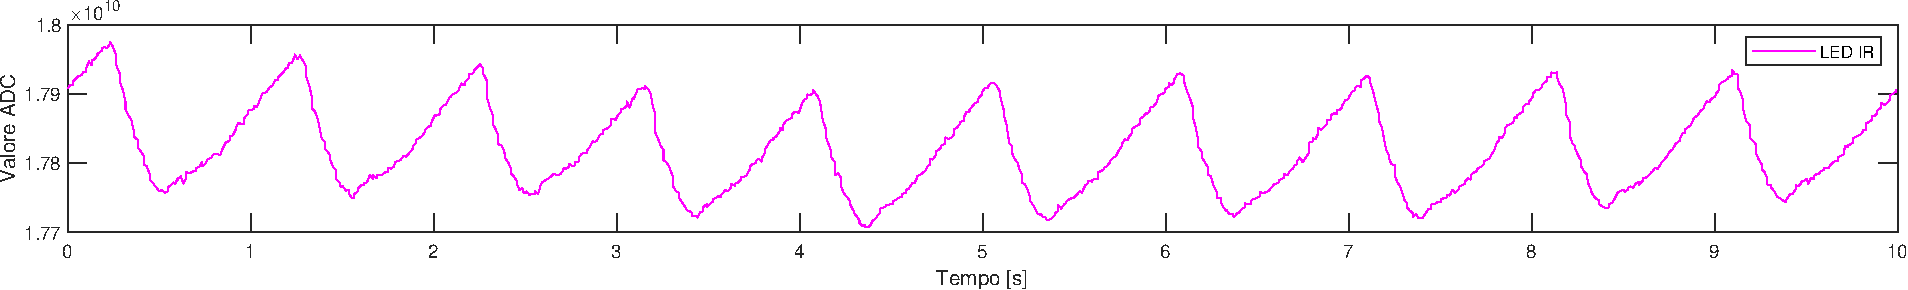
\includegraphics[width=1\linewidth]{ImageFiles/Misure Preliminari/Soggetto 1/lobo_ired}
	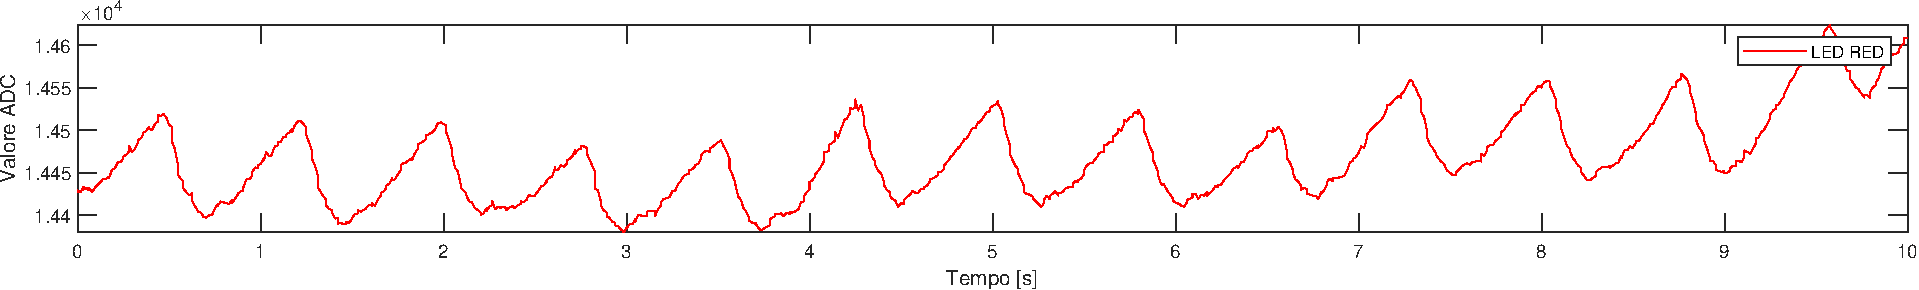
\includegraphics[width=1\linewidth]{ImageFiles/Misure Preliminari/Soggetto 1/lobo_red}
	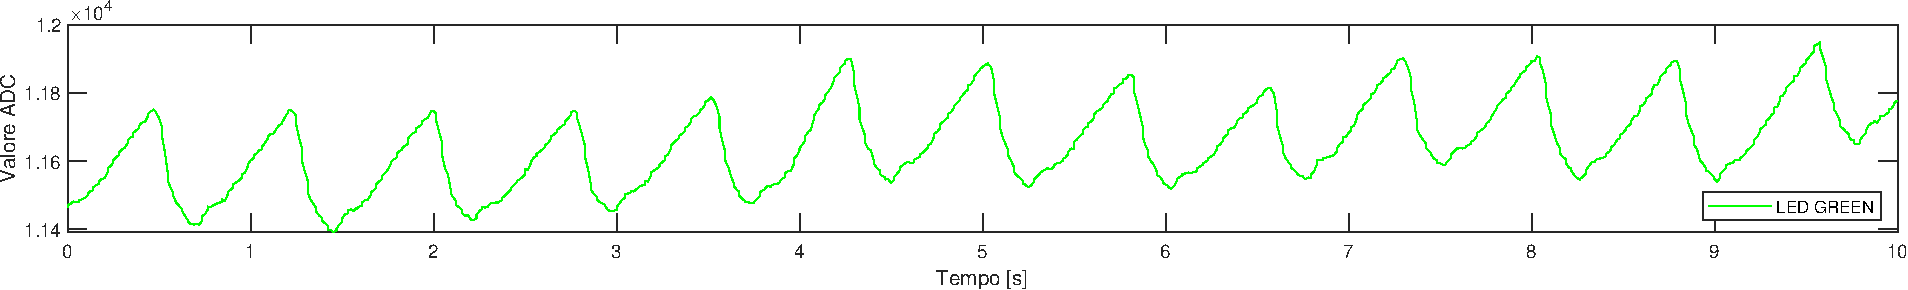
\includegraphics[width=1\linewidth]{ImageFiles/Misure Preliminari/Soggetto 1/lobo_green}
	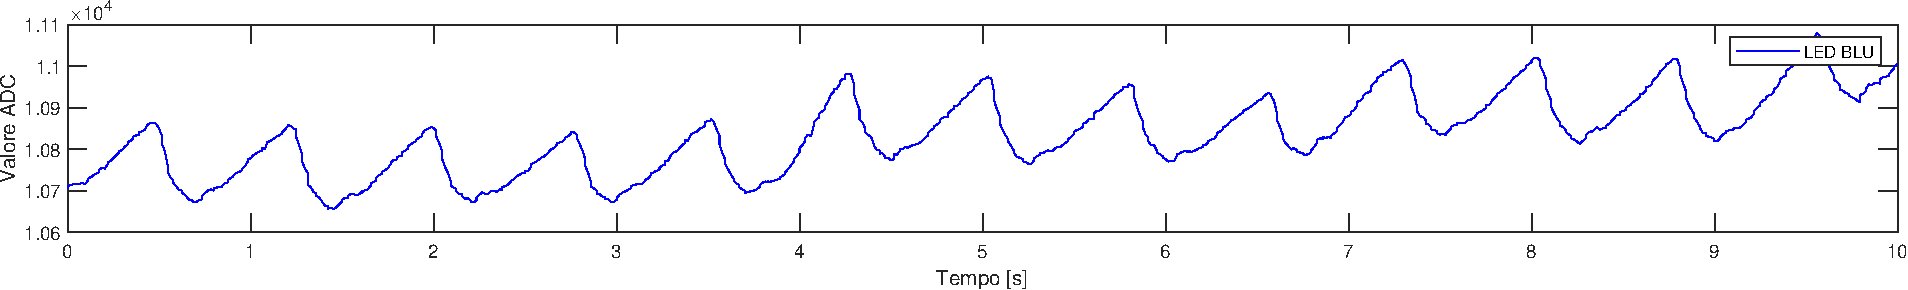
\includegraphics[width=1\linewidth]{ImageFiles/Misure Preliminari/Soggetto 1/lobo_blu}
	\caption{Segnali PPG acquisiti sul lobo dell'orecchio destro.}
	\label{fig:soggetto1_lobo}
\end{figure}

\clearpage

\subparagraph{Polso antero-interno}

Si sono eseguite anche delle misurazioni (\Fig~\ref{fig:oggetto1_polso}) sulla parte inferiore (antero-interna) del polso. Questa zona si è dimostrata molto disturbata dai movimenti del soggetto. I segnali del LED infrarosso e rosso risultano essere molto disturbati, sebbene siano ancora visibili i picchi caratteristici. I segnali dei LED verdi e blu risultano invece essere di buona qualità. La frequenza cardiaca che si può stimare è di 84 battiti al minuto. \todo{filtro sui dati}

\begin{figure}[h]
	\centering
	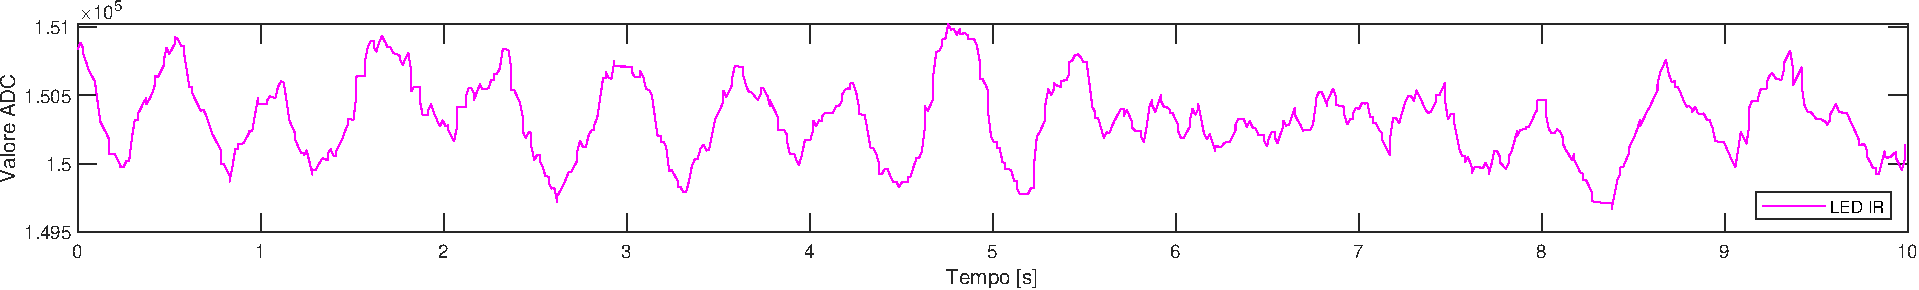
\includegraphics[width=1\linewidth]{ImageFiles/Misure Preliminari/Soggetto 1/polso_ired}
	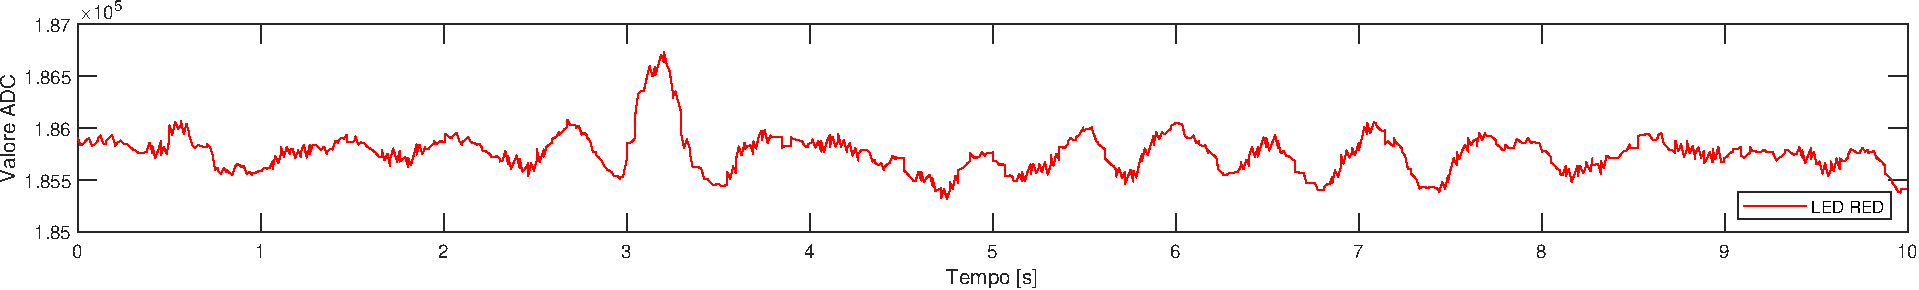
\includegraphics[width=1\linewidth]{ImageFiles/Misure Preliminari/Soggetto 1/polso_red}
	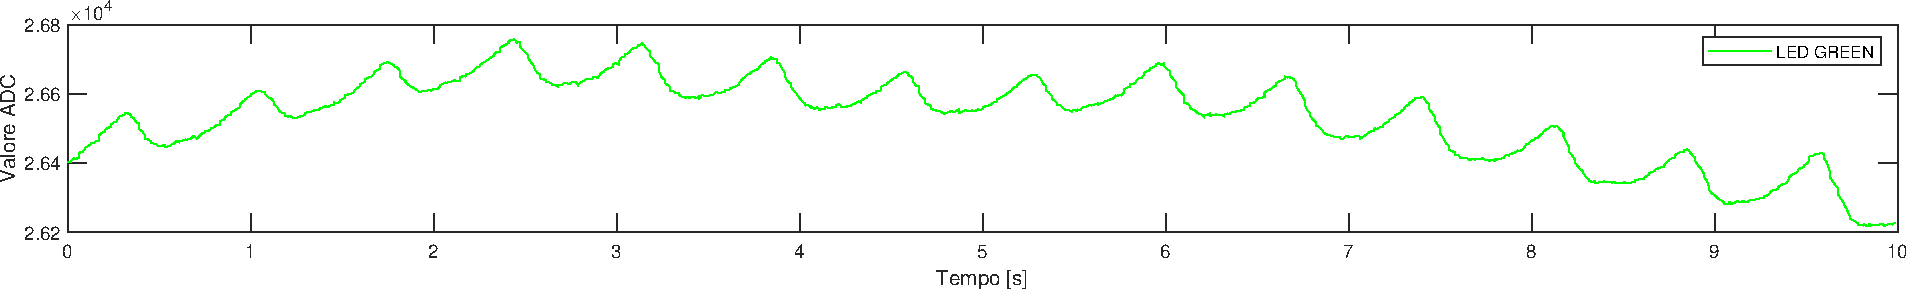
\includegraphics[width=1\linewidth]{ImageFiles/Misure Preliminari/Soggetto 1/polso_green}
	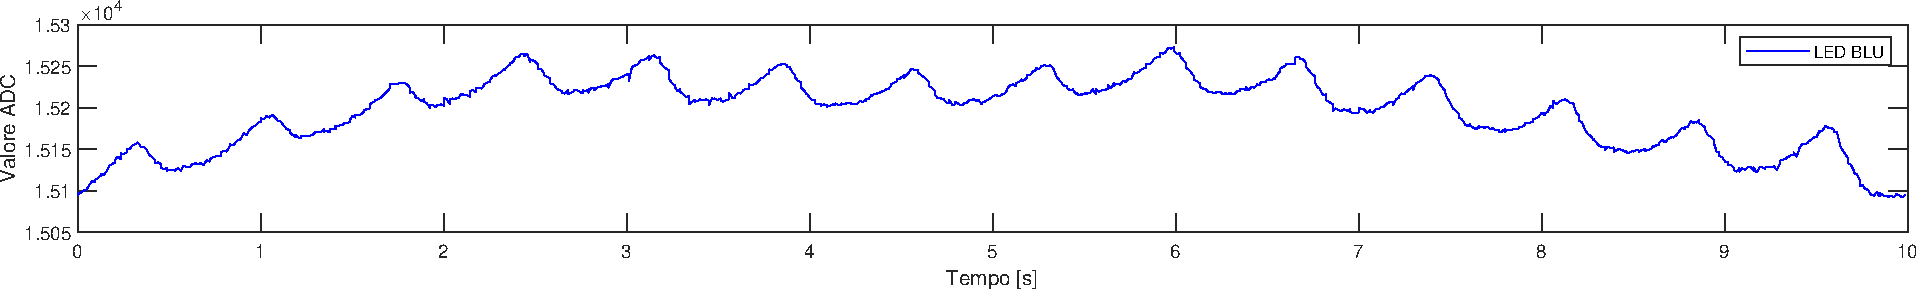
\includegraphics[width=1\linewidth]{ImageFiles/Misure Preliminari/Soggetto 1/polso_blu}
	\caption{Segnali PPG acquisiti sul polso destro.}
	\label{fig:soggetto1_polso}
\end{figure}

\clearpage

\subparagraph{Fronte}

L'ultimo sito di misura analizzato è la fronte (\Fig~\ref{fig:soggetto1_fronte}). A differenza degli altri siti di misura presentati, l'onda PPG è visibile solamente nelle acquisizioni dei LED infrarosso e rosso, rendendo inutilizzabile le misurazioni dei LED verdi e blu. Anche questo sito è poco influenzato dai movimenti del soggetto e potrebbe essere utilizzato per misurazioni durante l'attività fisica. Si può stimare una frequenza cardiaca del soggetto pari a 84 battiti al minuto.

\begin{figure}[h]
	\centering
	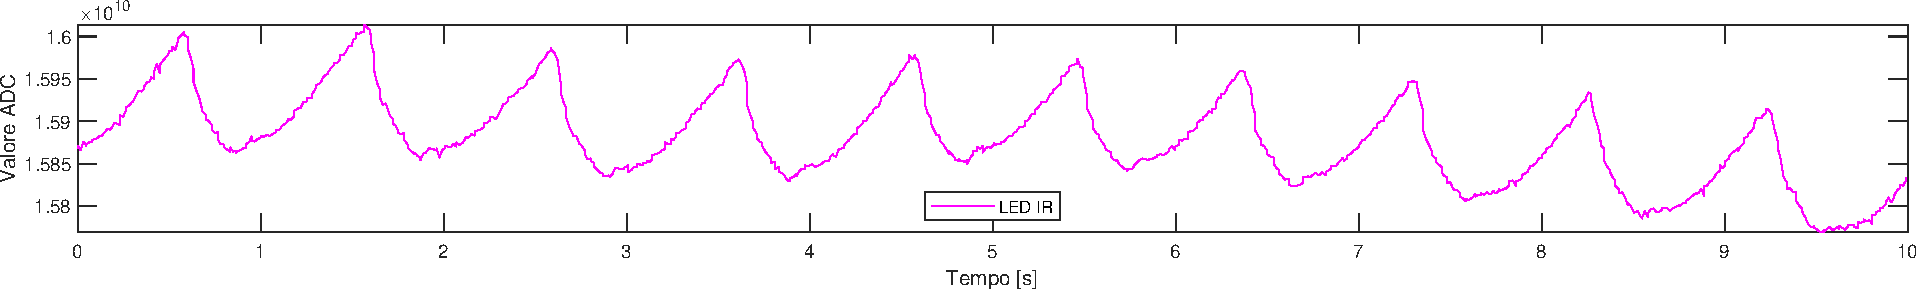
\includegraphics[width=1\linewidth]{ImageFiles/Misure Preliminari/Soggetto 1/fronte_ired}
	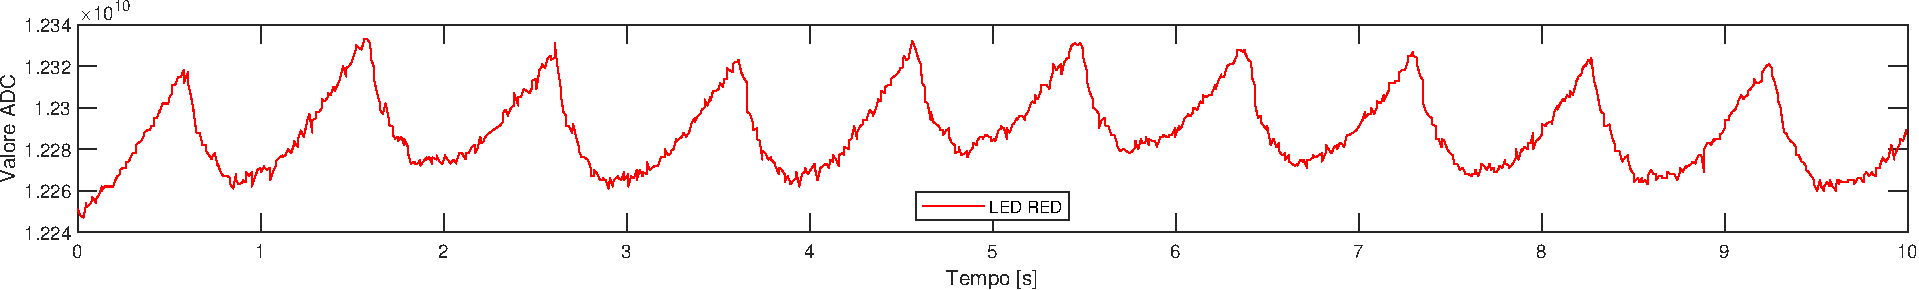
\includegraphics[width=1\linewidth]{ImageFiles/Misure Preliminari/Soggetto 1/fronte_red}
	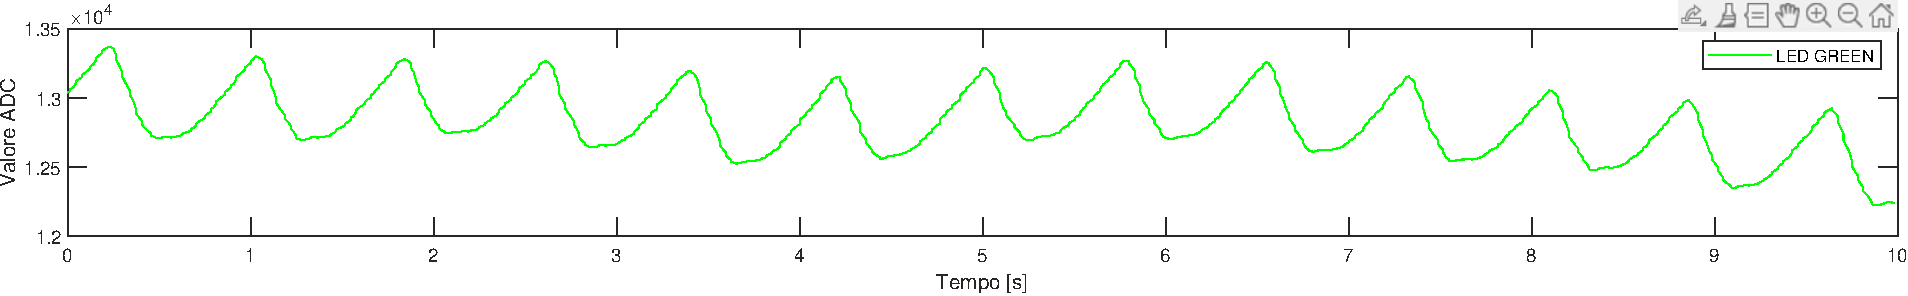
\includegraphics[width=1\linewidth]{ImageFiles/Misure Preliminari/Soggetto 1/fronte_green}
	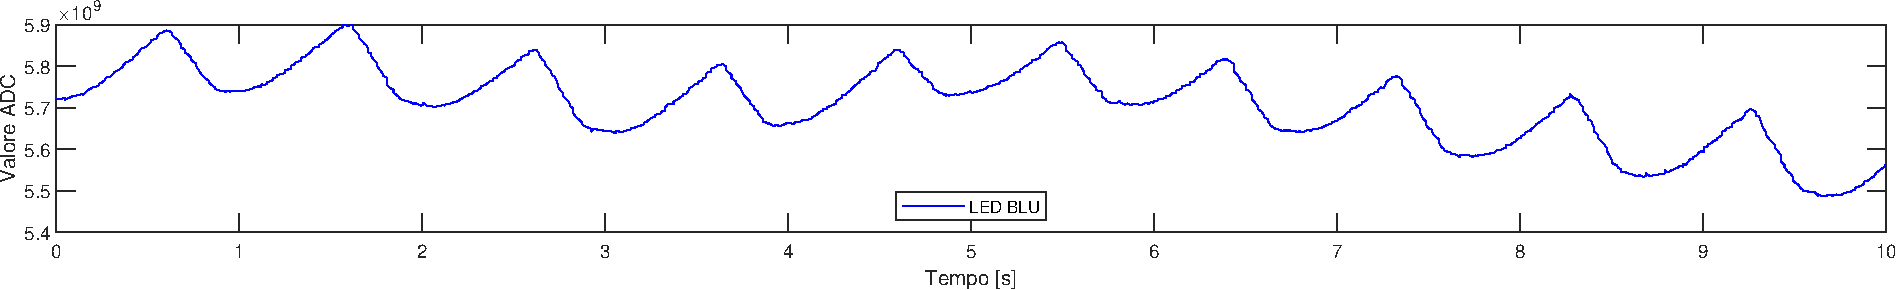
\includegraphics[width=1\linewidth]{ImageFiles/Misure Preliminari/Soggetto 1/fronte_blu}
	\caption{Segnali PPG acquisiti sulla fronte.}
	\label{fig:soggetto1_fronte}
\end{figure}






\clearpage